\documentclass[11pt, a4paper]{article}

\usepackage[margin=1in]{geometry}
\usepackage{graphicx}
\usepackage{amsmath, amssymb}
\usepackage{listings}
\usepackage{xcolor}
\usepackage{hyperref}
\usepackage{booktabs}
\usepackage{subcaption}
\usepackage{float}
\usepackage{fancyhdr}
\usepackage{enumitem}

\pagestyle{fancy}
\fancyhf{}
\fancyfoot[C]{\thepage}

\begin{document}

\fancypagestyle{no_hdr_border_rule}{
  \renewcommand{\headrulewidth}{0pt}
}
\thispagestyle{no_hdr_border_rule}

\begin{center}
    {\Large \textbf{Assignment 2 -- Report}} \\[0.2cm]
    {\large \textbf{Computing in Sciences -- I}} \\[0.1cm]
    {\normalsize International Institute of Information Technology, Hyderabad} \\[0.3cm]
\end{center}

\vspace{0.2cm}
\hrule
\vspace{0.4cm}

\noindent \textbf{Student Name:} Manbir Singh Judge \\
\noindent \textbf{Roll Number:} 2026112005 \\
\noindent \textbf{Protein:} 2HEP \\

\hrule
\vspace{0.5cm}

\vspace{1em}

\tableofcontents
\vspace{0.5cm}
\hrule
\vspace{0.8cm}

\newpage
\fancyhead[L]{CIS-I}
\fancyhead[R]{Assignment 2 -- Report}

\section{Part A -- Custom MD Engine}

\subsection{Part A1}
Starter file was completed including -- energy and forces for all five terms, periodic box and 9 \AA \space cutoff. \\
The code is present under the folder \verb|our_engine|.

\subsection{Part A2 -- Velocity Verlet and Plots}
The velocity Verlet loop was added in \verb|our_engine/engine.py|. \\
The simulation was run for 2 ps at 1 fs. \\
Following are the plots: 

\begin{figure}[H]
    \centering

    \begin{subfigure}{0.48\textwidth}
        \centering
        \includegraphics[width=\textwidth]{our_engine/out/K_0.5.png}
    \end{subfigure}
    \hfill
    \begin{subfigure}{0.48\textwidth}
        \centering
        \includegraphics[width=\textwidth]{our_engine/out/K_1.0.png}
    \end{subfigure}

    \vspace{0.5cm}

    \begin{subfigure}{0.48\textwidth}
        \centering
        \includegraphics[width=\textwidth]{our_engine/out/P_0.5.png}
    \end{subfigure}
    \hfill
    \begin{subfigure}{0.48\textwidth}
        \centering
        \includegraphics[width=\textwidth]{our_engine/out/P_1.0.png}
    \end{subfigure}

    \vspace{0.5cm}

    \begin{subfigure}{0.48\textwidth}
        \centering
        \includegraphics[width=\textwidth]{our_engine/out/E_0.5.png}
    \end{subfigure}
    \hfill
    \begin{subfigure}{0.48\textwidth}
        \centering
        \includegraphics[width=\textwidth]{our_engine/out/E_1.0.png}
    \end{subfigure}
\end{figure}

Change in total energy:
\begin{itemize}[leftmargin=1.5cm]
    \item \textbf{For dt = 0.5 fs:} 2.716 kcal/mol
    \item \textbf{For dt = 1 fs:} 81.718 kcal/mol
    \item \textbf{For dt = 2 fs:} -
\end{itemize}

\textbf{Note:} The simulation didn't complete for \verb|dt = 2 fs|. The reason is discussed later.

% \subsection{Part A3}
% \begin{table}[H]
%     \centering
%     \begin{tabular}{|c|c|c|c|}
%         \hline
%         $S$ & $R/W$ & Operation & Output \\
%         \hline
%         0 & X & None & 0 \\
%         \hline
%         1 & 0 & Read & Q \\
%         \hline
%         1 & 1 & Write & 0 \\
%         \hline
%     \end{tabular}
% \end{table}

\subsection{Part A4 -- Comparing Energy Fluctuation}

\begin{figure}[H]
    \centering
    \includegraphics[width=0.75\textwidth]{our_engine/out/E_fluctuation_0.5.png}
\end{figure}

\begin{figure}[H]
    \centering
    \includegraphics[width=0.75\textwidth]{our_engine/out/E_fluctuation_1.0.png}
\end{figure}

We see that energy fluctuation is a lot less when \verb|dt = 0.5 fs| as compared to \verb|dt = 1 fs|. The reason behind this is -- we are using Taylor series expansion and removing higher degree terms in our Verlet integrator. This is required to make the equations computationally solvable. But, it introduces errors which accumulate overtime. Magnitude of errors depends on \verb|dt|. Hence, that error is less in case of \verb|dt = 0.5 fs|.

\section{Part B -- NAMD and OpenMM Simulations}
Run \verb|namd/run.sh| to run NAMD simulations for all three timesteps. \\
The provided OpenMM simulation scripts were used as-is. \\
The provided analysis scripts for Part B were also used without any changes.

\subsection{Plots}

\begin{figure}[H]
    \centering
    \includegraphics[width=\textwidth]{part_b/out/nve_2HEP_dt0.5.png}
    \caption{Plots for dt = 0.5 fs}
\end{figure}

\begin{figure}[H]
    \centering
    \includegraphics[width=\textwidth]{part_b/out/nve_2HEP_dt1.png}
    \caption{Plots for dt = 1 fs}
\end{figure}


\subsection{Statistics}
\begin{table}[H]
    \centering
    \begin{tabular}{|c|c|c|c|c|}
        \hline
        Engine & dt (fs) & $\langle T \rangle$ (K) & $\langle E \rangle$ (kcal/mol) & Drift (kcal/ns) \\
        \hline
        NAMD & 0.5 & 320.95 & -29773.10 & 200.96 \\
        \hline
        NAMD & 1.0 & 315.33 & -29702.43 & -51.09 \\
        \hline
        NAMD & 2.0 & \multicolumn{3}{c|}{Simulation did not complete} \\
        \hline
        OpenMM & 0.5 & 307.32 & -24707.27 & 353.46 \\
        \hline
        OpenMM & 1.0 & 301.79 & -24634.19 & 521.022 \\
        \hline
        OpenMM & 2.0 & \multicolumn{3}{c|}{Simulation did not complete} \\
        \hline
    \end{tabular}
    \caption{Comparison of Statistics NAMD and OpenMM simulations}
\end{table}

\subsection{Discussion}
Kinetic and potential energy mirror each other because total energy is conserved.\\
Temperature fluctuates because potential and kinetic energies are continuously being exchanged with each other. And change in kinetic energy leads to change in temperature.

\subsection{VMD Visualization}

\begin{figure}[H]
    \centering

    \begin{subfigure}{0.48\textwidth}
        \centering
        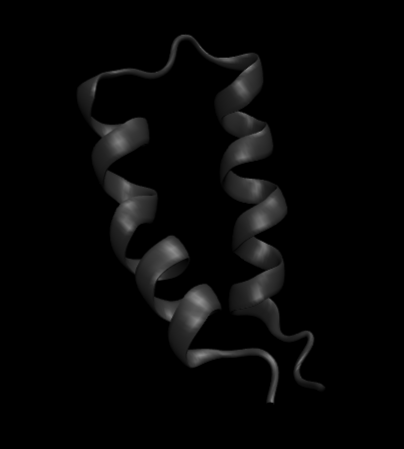
\includegraphics[width=\textwidth]{vmd_vis.png}
        \caption{VMD Visualization -- Ribbons}
    \end{subfigure}
    \hfill
    \begin{subfigure}{0.48\textwidth}
        \centering
        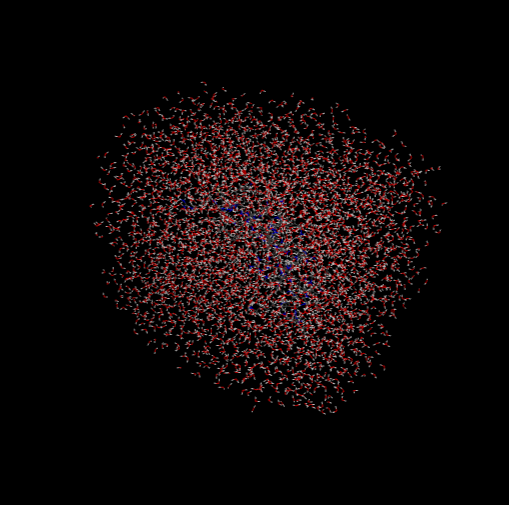
\includegraphics[width=\textwidth]{vmd_wb.png}
        \caption{VMD Visualization -- Water Box}
    \end{subfigure}
\end{figure}

\section{Part C -- Comparing the Engines}

\subsection{Starting Structure: Potential Energy Comparison}

The potential energy of the starting protein structure was calculated
using all three engines. The energy components are compared below.
All values are expressed in kcal/mol.

\begin{table}[h]
    \centering
    \caption{Potential energy components of the starting structure}
    \begin{tabular}{lrrr}
        \hline
        \textbf{Energy Component} &
        \textbf{Our Engine} &
        \textbf{NAMD} &
        \textbf{OpenMM} \\
        \hline
        Bond             &  &  &  \\
        Angle            &  &  &  \\
        Dihedral         &  &  &  \\
        van der Waals    &  &  &  \\
        Electrostatic    &  &  &  \\
        \hline
        Total Potential  & & & \\
        \hline
    \end{tabular}
    \label{tab:potential_energy}
\end{table}

The bond and angle energy terms show agreement. The differences may arise
from variations in force-field implementations, non-bonded interaction
cutoffs, parameter handling and numerical approximations.

\subsection{NVE Simulation: Energy Conservation}

The three engines were compared using their 2 ps NVE simulations.
The total energy was monitored throughout each simulation to evaluate
energy fluctuations and drift.

\begin{table}[H]
    \centering
    \caption{Total energy statistics for the 2 ps NVE simulations}
    \begin{tabular}{lrrr}
        \hline
        \textbf{Quantity} &
        \textbf{Our Engine} &
        \textbf{NAMD} &
        \textbf{OpenMM} \\
        \hline
        Initial Energy (kcal/mol) &  &  & \\
        Final Energy (kcal/mol)   &  &  & \\
        Minimum Energy (kcal/mol) &  &  & \\
        Maximum Energy (kcal/mol) &  &  & \\
        Fluctuation (kcal/mol)    &  &  & \\
        Energy Drift (kcal/mol)   &  &  & \\
        \hline
    \end{tabular}
    \label{tab:nve_energy}
\end{table}

NAMD showed the best energy conservation. Differences between the engines may be attributed
to numerical integration errors, timestep selection and differences
in force calculations.

A sharp cutoff in nonbonded interactions can introduce energy drift.
When particles cross the cutoff distance, the interaction energy
changes discontinuously. This introduces artificial changes in the
total energy. Switching functions or shifted potentials can reduce
this problem.

\subsection{Conclusion}

The comparison of the three engines provides insight into the
accuracy of the force-field calculations and the stability of their
molecular dynamics simulations.

All initial energies agree quite closely for all engines. 

NVE had the best performance. 

Our implementation successfully reproduced most value. However, it showed limitations in
cutoff implementation (and performance, but we won't discuss that here). These differences
highlight the importance of accurate force calculations and
numerical integration.

\section{Part D -- About the Protein}
The protein selected for this simulation is YnzC (UPF0291) from \textit{Bacillus subtilis}, a Gram-positive bacterium. It belongs to the DUF896 protein family, whose biological function is not yet fully understood. The \textit{ynzC} gene is involved in the bacterial SOS response, which is activated when DNA is damaged. However, the exact biological role of YnzC remains unknown \cite{rcsb_2hep,uniprot_ynzc}.

Structurally, YnzC is a relatively small protein with 77 amino acids
in its natural sequence. Its experimentally determined structure
(PDB: 2HEP) was obtained using solution NMR rather than X-ray
crystallography. The folded region consists primarily of two
antiparallel alpha helices connected by a loop (a helix-loop-helix
motif). The remaining C-terminal region is largely disordered in
solution. The deposited structure contains 42 ordered residues
\cite{rcsb_2hep,uniprot_ynzc}.

This protein is interesting for molecular dynamics simulations
because of its small size and relatively simple structure. It provides
an opportunity to study the behaviour of stable secondary structures
alongside disordered regions. Its NMR structure also makes it useful
for studying protein conformations and testing molecular simulation
methods.

In our simulation, the protein was placed in an explicit solvent
environment, with counterions added to neutralize its net charge.
The protein had a total charge of 0, and 3 ions were added. The simulation was performed
for 12 ps. However, this duration is too short to observe meaningful
biological processes or determine the protein's actual function.
Instead, it is mainly useful for examining short-timescale structural
stability, atomic motion and energy conservation.

\begin{thebibliography}{9}
\bibitem{rcsb_2hep}
RCSB Protein Data Bank, ``PDB ID: 2HEP'',
\url{https://www.rcsb.org/structure/2HEP}.

\bibitem{uniprot_ynzc}
UniProt, ``YnzC (UPF0291), Bacillus subtilis'',
\url{https://www.uniprot.org/uniprotkb/O31818/entry}.
\end{thebibliography}


\end{document}